\chapter{State of the Art}
\chaptermark{State of the Art}
\label{chapter:soa}
\minitoc

%%%%%%%%%%%%%%%%%%%%%%%%%%%%%%%%%%%%%%%%%%%%%%%%%%%%%%%%%%%%%%%%%%%%%%%%%%%%%%%%%%%%%%%%%%%%%%%
\section{Introduction}
This chapter provides an overview of related work to contextualize the primary objectives of this thesis. Firstly, in Section~\ref{section:ift}, Information Flow Tracking (IFT) is introduced, detailing the different types and their respective purposes. We will discuss the various levels of monitoring, from program behaviour to the detection of hardware trojans.
Then in Section~\ref{section:physicalAttacks}, Physical Attacks are examined, focusing on two main types: Side-Channel Attacks (SCA) and Fault Injection Attacks (FIA).
Finally in Section~\ref{section:countermeasuresAgainstFIA}, as this work will concentrate on FIA, we will exclusively present countermeasures against Fault Injection Attacks.

%%%%%%%%%%%%%%%%%%%%%%%%%%%%%%%%%%%%%%%%%%%%%%%%%%%%%%%%%%%%%%%%%%%%%%%%%%%%%%%%%%%%%%%%%%%%%%%
\section{Information Flow Tracking}
\label{section:ift}
This section introduces Information Flow Tracking mechanisms, explains how they work, and presents the various types of IFT with their different functional levels.
% We mainly focus on presenting hardware IFT architectures.
    
%%%%%%%%%%%%%%%%%%%%%%%%%%%%%%%%
\subsection{Different types of IFT}
There are two distinct types of IFT approaches: static and dynamic, each with its own specific objectives.

\subsubsection{Static IFT}
Static Information Flow Tracking (SIFT) is a security technique used to analyse and control the flow of information within a program or system without executing it, by examining the source code or compiled binary~\cite{HAK-21-acmcsur}. This method is particularly useful for identifying theoretical vulnerabilities, ensuring compliance with design principles, and preventing unauthorised information leaks before deployment. SIFT is comprehensive, covering all possible execution paths and detecting both explicit information flows (direct data assignments) and implicit flows (leaks through control flow structures). By performing checks at compile-time, SIFT helps developers address potential security issues early, enforcing principles like non-interference and data confidentiality through security policies. However, static analysis may generate false positives by flagging theoretical flows that might not occur in practice and may struggle with certain dynamic language features or runtime-dependent behaviours. SIFT is employed in various contexts, such as verifying secure information flow in operating systems, programming languages with built-in information flow controls, and hardware design for secure systems.

\subsubsection{Dynamic IFT}
Dynamic Information Flow Tracking (DIFT) is a powerful security technique that monitors and analyses, in real-time, the flow of information within a program during its execution~\cite{CGDJ-21-micromac}. DIFT operates by tagging or labelling input data from potentially untrusted sources and tracking how this data propagates through the system~\cite{SLD-04-sigplan}. As the program executes, DIFT maintains metadata about the tagged information, updating it as operations are performed on the data. This allows the system to detect when tainted data is used in security-critical operations, such as modifying control flow or accessing sensitive resources. DIFT can be implemented at various levels, including hardware, software, or a combination of both. Hardware-based implementations often offer better performance but require specialized processor modifications, while software-based approaches provide more flexibility but may incur higher overhead~\cite{CGDJ-21-micromac}. DIFT has proven effective in detecting and preventing a wide range of security vulnerabilities, including buffer overflows, format string attacks, and code injection attacks~\cite{SLD-04-sigplan}. However, DIFT also faces challenges, such as handling implicit information flows, managing performance overhead, and addressing over-tainting issues.
This approach might not cover all potential data paths, as it is dependent on the specific conditions and inputs provided during the monitoring period.
Despite these challenges, DIFT remains a valuable tool in the cybersecurity arsenal, particularly for runtime attack detection and prevention in modern computing systems.

%%%%%%%%%%%%%%%%%%%%%%%%%%%%%%%%    
\subsection{Different levels of IFT}
IFT can be implemented at various levels of abstraction in computing systems. Each level presents unique trade-offs between precision, performance overhead, and ease of implementation, allowing designers to choose the most appropriate approach for their security requirements.
At the lowest level, Gate-Level IFT (GLIFT) tracks information flow through individual logic gates, providing precise security guarantees.
Moving up, Register Transfer Level IFT (RTLIFT) operates on hardware descriptions, enabling early-stage verification of security properties.
At the microarchitecture level, IFT can be implemented within processor cores or as off-core designs, balancing performance and security.
Software-based IFT operates at either the system level, monitoring OS-wide information flows, or the program level, focusing on specific applications.
Finally, hardware-software co-designed IFT solutions aim to leverage the strengths of both hardware and software implementations.

Figure~\ref{fig:levels_system} represents the four different levels of a simplified embedded system: application layer, system service layer, OS layer, and hardware layer. This figure is inspired by Figure 1.9 of~\cite{ebrary}.

Positioned at the highest level of the software hierarchy, \textit{the application layer} is responsible for implementing system functionalities and business logic. Functionally, all modules within this layer work together to execute the required system operations. Applications generally run in a less-privileged mode on the processor and utilise the OS-provided API scheduling to communicate with the operating system.
\textit{The system service layer} serves as the intermediary service interface offered by the OS to the application layer. This interface allows applications to access a variety of OS-provided services, essentially bridging the gap between the OS and applications. Typically, this layer encompasses components like the file system, Graphical User Interface (GUI), task manager.
An Operating System (OS) is a software framework designed to manage hardware resources uniformly. It abstracts numerous hardware functions and offers them to applications as services. Common services provided by an OS include scheduling, file synchronisation, and networking. Operating systems are prevalent in both desktop and embedded systems. In the context of embedded systems, OSs possess distinct characteristics such as stability, customisability, modularity, and real-time processing capabilities.
\textit{The hardware layer} refers to the physical components and circuitry, including the microprocessor or microcontroller, memory, sensors, and input/output interfaces. This layer encompasses all the tangible electronic elements that interact directly with each other to perform the device's functions. It provides the essential infrastructure that supports and drives the embedded system’s operations and connectivity.

\begin{figure}[ht]
    \centering
    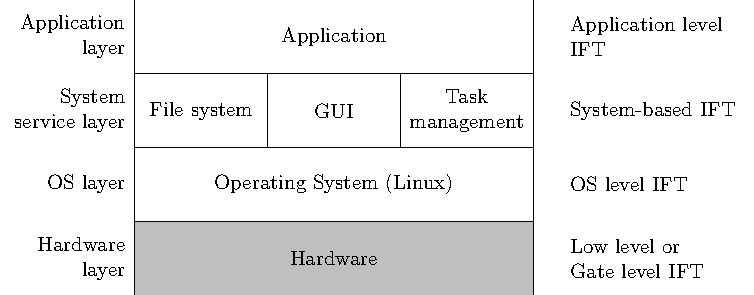
\includegraphics{c2_soa/img/system_layer.pdf}
    \caption{Simplified representation of the different layers in an embedded system}
    \label{fig:levels_system}
\end{figure}

Tracking information can be performed at various levels, from the application level to the hardware level. Each level offers distinct advantages and disadvantages.
%For instance, application-level tracking might provide detailed insights and user-friendly interfaces, while hardware-level tracking offers more granular data and real-time monitoring but can be more complex and costly.
The following subsections will explore these different levels, highlighting their respective benefits and limitations.

\subsubsection{Application level IFT}
Application level IFT tracks information flows between application variables. The programmer has to integrate data tagging inside his program and use a modified compiler or analyse his program to check if no security violation happened.


\subsubsection{OS level and System-based IFT}
\subsubsection{Low level IFT}

%%%%%%%%%%%%%%%%%%%%%%%%%%%%%%%%
\subsection{DIFT Architectures}
\subsubsection{Off-Core}

\subsubsection{Off-Loading}

\subsubsection{In-Core}

%%%%%%%%%%%%%%%%%%%%%%%%%%%%%%%%
\subsection{How DIFT works}
\wip{expliquer DIFT ici ? en détail avec les schémas explicatifs}

%%%%%%%%%%%%%%%%%%%%%%%%%%%%%%%%%%%%%%%%%%%%%%%%%%%%%%%%%%%%%%%%%%%%%%%%%%%%%%%%%%%%%%%%%%%%%%%
\section{Physical Attacks}
\label{section:physicalAttacks}

\subsection{Side-Channel Attacks}
\subsection{Fault Injection Attacks}
% A fault is the cause of an error, that is, an incorrect program or circuit state. If the error caused by the fault does not propagate and the application execution ends normally, the fault is ineffective. On the contrary, the fault is effective if the error affects the application’s execution, causing a failure, an observed behavior different from that expected.
% In the context of electronic circuits, a fault refers to an unintended deviation from the normal operation of the circuit. Faults can occur due to various reasons such as manufacturing defects, environmental factors, ageing, or external interference. These faults can affect the performance, functionality, and reliability of the circuit.

% In fault injection, which is a testing method used to evaluate the robustness and reliability of electronic circuits, a fault is deliberately introduced into the system to observe its behaviour and identify potential vulnerabilities.

%%%%%%%%%%%%%%%%%%%%%%%%%%%%%%%%%%%%%%%%%%%%%%%%%%%%%%%%%%%%%%%%%%%%%%%%%%%%%%%%%%%%%%%%%%%%%%%
\section{Countermeasures against FIA}
\label{section:countermeasuresAgainstFIA}

%%%%%%%%%%%%%%%%%%%%%%%%%%%%%%%%%%%%%%%%%%%%%%%%%%%%%%%%%%%%%%%%%%%%%%%%%%%%%%%%%%%%%%%%%%%%%%%